\subsection{ORES system engineering}
\label{sec:ores_system_engineering}
In this section we describe how the system was designed in order to meet the needs of Wikipedian work practices and the tools that support them.

\subsubsection{Scaling \& robustness}
To be useful for Wikipedians and tool developers, ORES uses distributed computation strategies to provide a robust, fast, high-availability service.  Reliability is a critical concern in Wikipedian quality control work.  Interruptions in Wikipedia's algorithmic systems have historically led to increased burdens for human workers and a higher likelihood that readers will see vandalism\cite{geiger2013levee}.  Further, ORES needs to scale to be able to be used in multiple different tools across different language Wikipedias where its predecessors only needed to scale for use in a single tool.

This horizontal scaleability is achieved in two ways: input-output (IO) workers (uwsgi\footnote{\url{https://uwsgi-docs.readthedocs.io/}}) and the computation (CPU) workers (celery\footnote{\url{http://www.celeryproject.org/}}).  Requests are split across available IO workers, and all necessary data is gathered using external APIs (e.g. the MediaWiki API\footnote{\url{http://enwp.org/:mw:MW:API}}).  The data is then split into a job queue managed by \emph{celery} for the CPU-intensive work.  This efficiently uses available resources and can dynamically scale, adding and removing new IO and CPU workers in multiple datacenters as needed.  This is also fault-tolerant, as servers can fail without taking down the service as a whole.

\subsubsection{Real-time processing}
The most common use case of ORES is real-time processing of edits to Wikipedia immediately after they are saved.  For example, those using counter-vandalism tools like Huggle monitor edits within seconds of when they are made.  It is critical that ORES return these requests in a timely manner.  We implement several strategies to optimize this request pattern.

\leadin{Single score speed}
In the worst case scenario, ORES is generating a score from scratch.  This is the common case when a score is requested in real-time---which invariably occurs right after the target edit or article is saved.  We work to ensure that the median score duration is around 1 second so that counter-vandalism efforts are not substantially delayed(c.f. \cite{geiger2013levee}).  Our metrics tracking currently suggests that for the week April 6-13th, 2018, our median, 75\%, and 95\% score response timings are 1.1, 1.2, and 1.9 seconds respectively.

\leadin{Caching and precaching}
In order to take advantage of our users' overlapping interests in scoring recent activity, we also maintain a basic least-recently-used (LRU) cache\footnote{Implemented natively by Redis, \url{https://redis.io}} using a deterministic score naming scheme (e.g. \texttt{enwiki:123456:damaging} would represent a score needed for the English Wikipedia damaging model for the edit identified by 123456).  This allows requests for scores that have recently been generated to be returned within about 50ms via HTTPS.  In other words, a request for a recent edit that had previously been scored is 20X faster due to this cache.

In order to make sure that scores for \emph{all recent edits} are available in the cache for real-time use cases, we implement a ``precaching'' strategy that listens to a high-speed stream of recent activity in Wikipedia and automatically requests scores for a specific subset of actions (e.g. edits).  With our LRU and precaching strategy, we consistently attain a cache hit rate of about 80\%.

\leadin{De-duplication}
In real-time ORES use cases, it's common to receive many requests to score the same edit/article right after it was saved.  We use the same deterministic score naming scheme from the cache to identify scoring tasks, and ensure that simultaneous requests for that same score are de-duplicated.  This allows our service to trivially scale to support many different robots and tools on the same wiki.

\subsubsection{Batch processing}
Many different types of Wikipedia's bots rely on periodic, batch processing strategies to support Wikipedian work processes\cite{geiger2011lives}.  For example, many bots are designed to build worklists for Wikipedia editors (e.g. \cite{cosley2007suggestbot}) on a daily or weekly basis, and many of these tools have adopted ORES to include an article quality prediction for use in prioritization of work (see section~\ref{sec:adoption_patterns}).  Work lists are either built from the sum total of all 5m+ articles in Wikipedia, or from some large subset specific to a single WikiProject (e.g. WikiProject Women Scientists claims about 6k articles\footnote{As demonstrated by \url{https://quarry.wmflabs.org/query/14033}}).  We've observed robots submitting large batch processing jobs to ORES once per day.  It's relevant to note that many researchers are also making use of ORES for various analyses, and their activity usually shows up in our logs as a similar burst of requests.

In order to most efficiently support this type of querying activity, we implemented batch optimizations in ORES by splitting IO and CPU operations into distinct stages.  During the IO stage, all data is gathered for all relevant scoring jobs in batch queries.  During the CPU stage, scoring jobs are split across our distributed processing system.  This batch processing affords up to a 5X increase in time to scoring speed for large requests\cite{sarabadani2017building}.  At this rate, a user can request 10s of million of scores in less than 24 hours in the worst case scenario (no scores were cached) without substantially affecting the service for others.

\subsubsection{Empirical access patterns}
\label{sec:appendix.empirical_access_patterns}
\begin{figure}[h]
\centering
\begin{subfigure}[t]{\columnwidth}
  \centering
  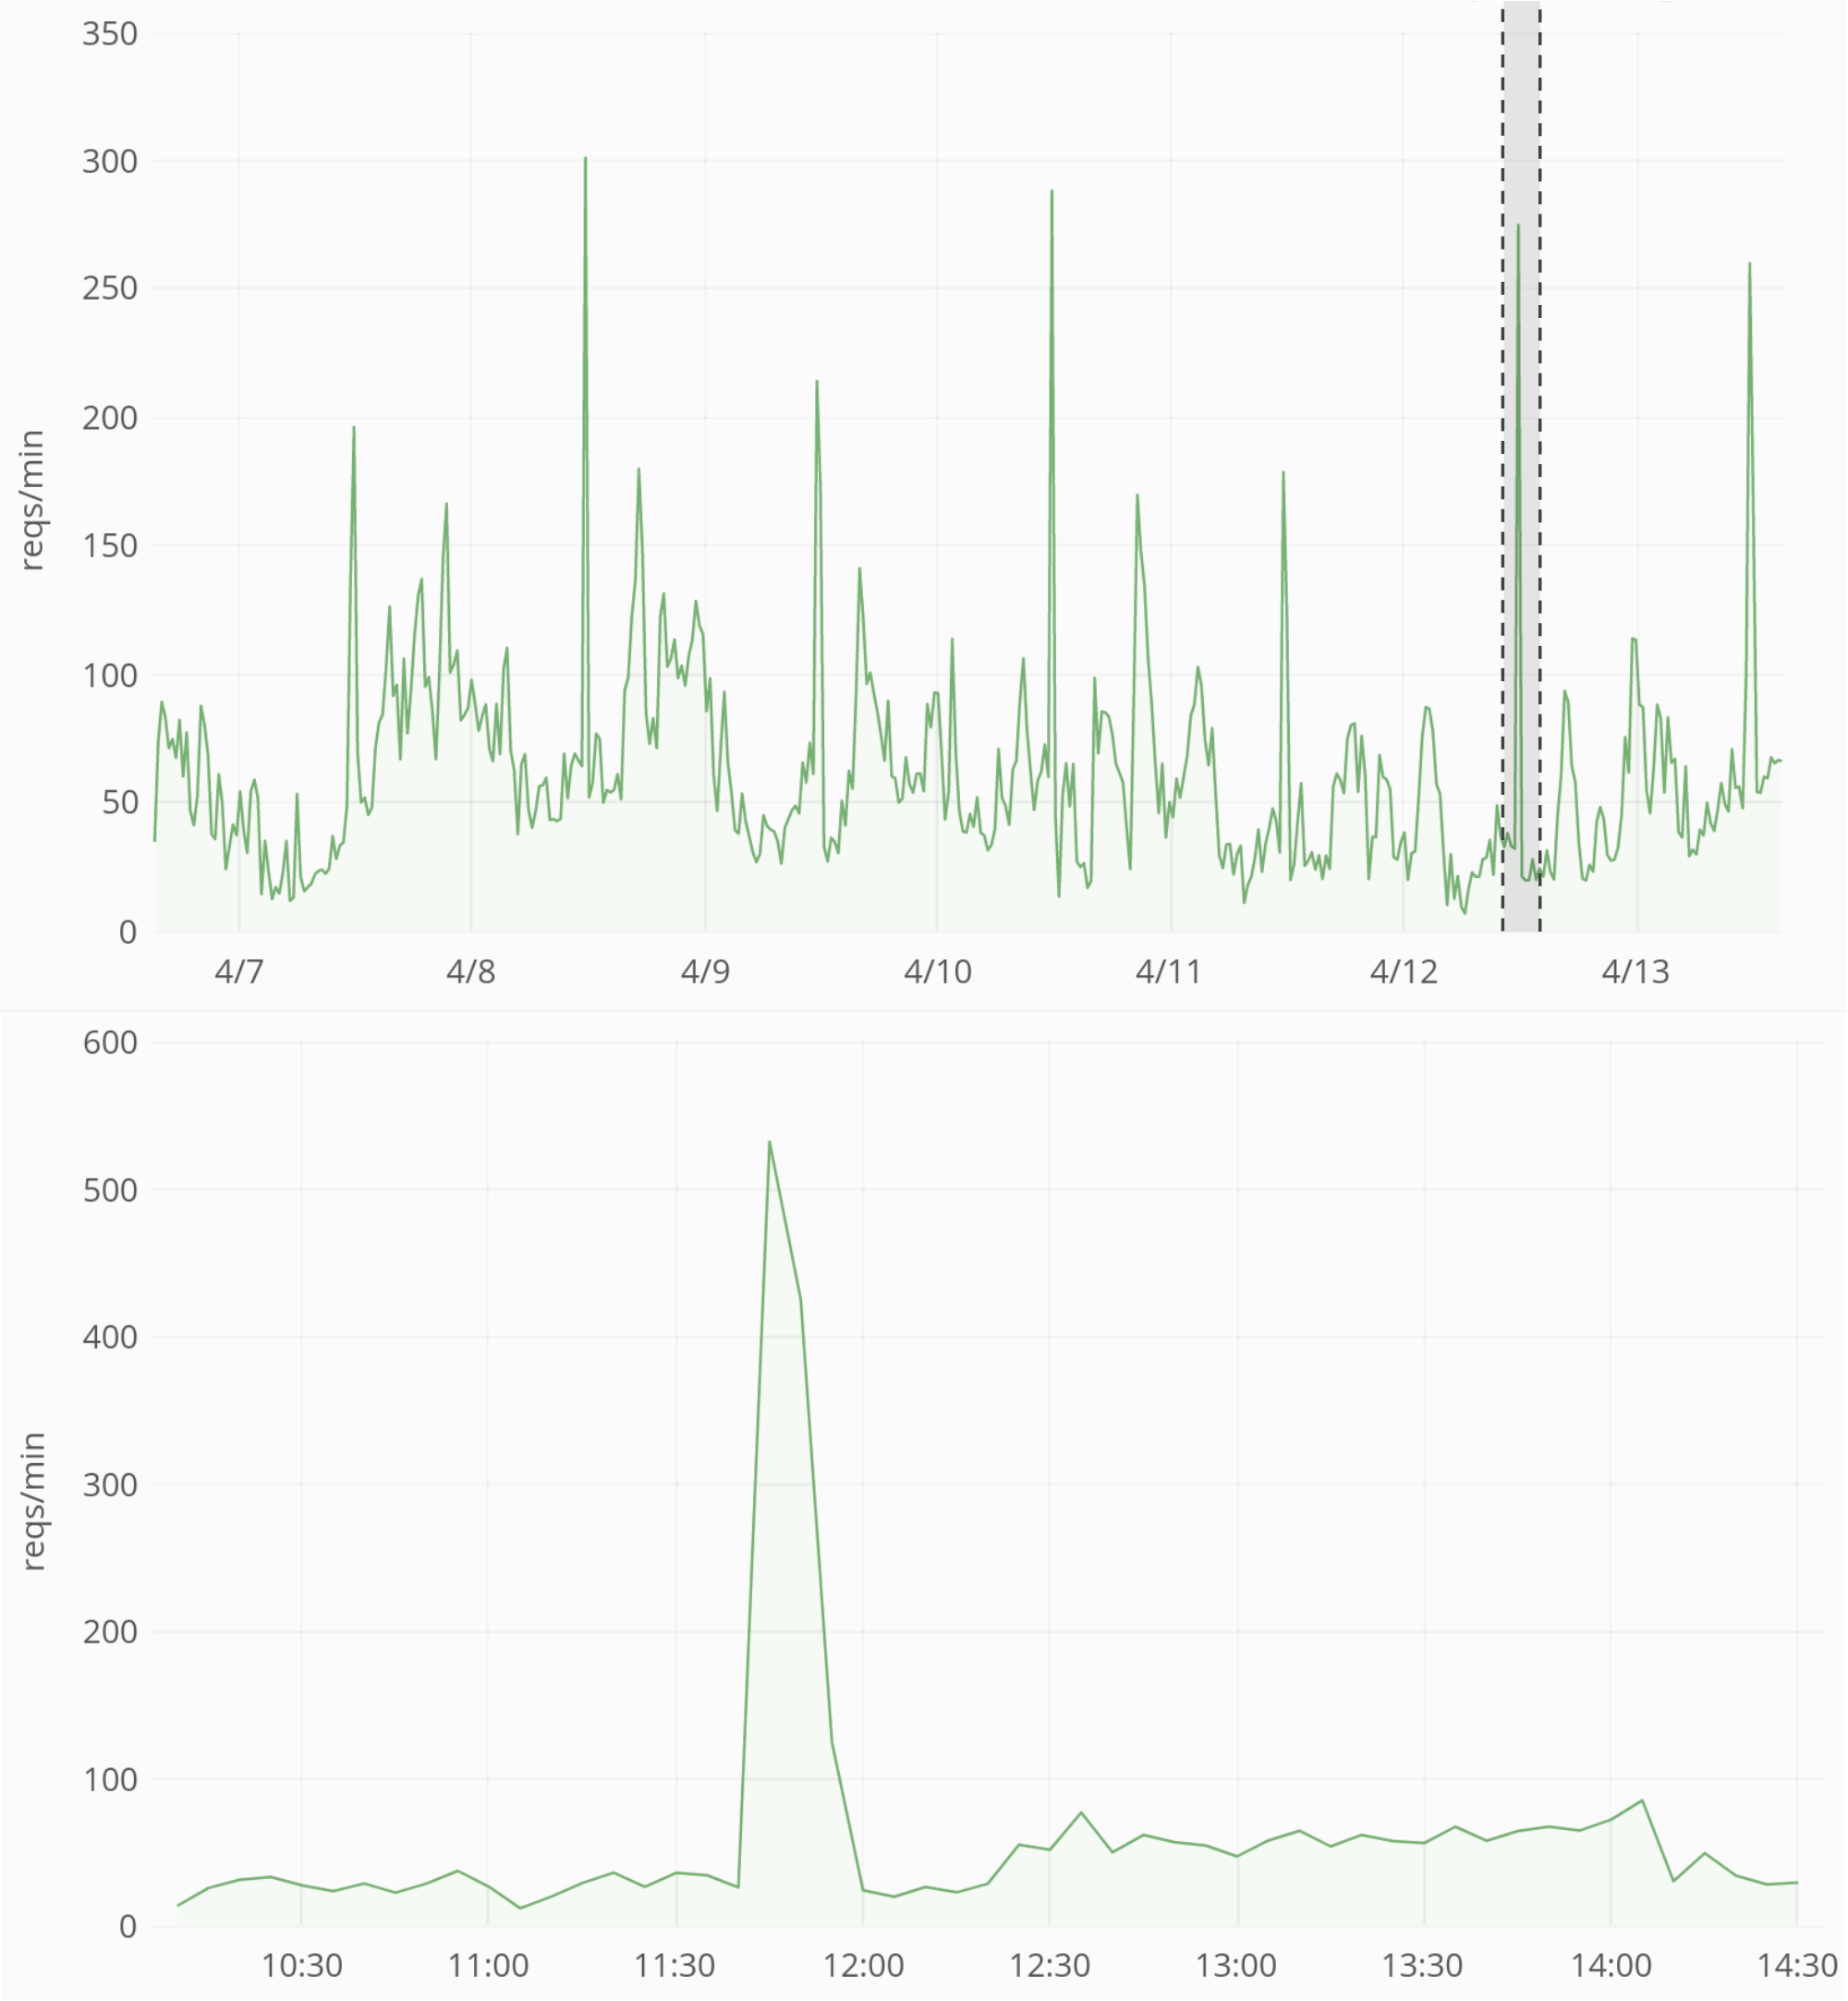
\includegraphics[width=.95\textwidth]{figures/ORES_request_activity_201804_week_vs_4hours}
  \caption{External requests per minute with a 4 hour block broken out to highlight a sudden burst of requests}
  \label{fig:ores_request_rate}
\end{subfigure}\\
\begin{subfigure}[t]{\columnwidth}
  \centering
  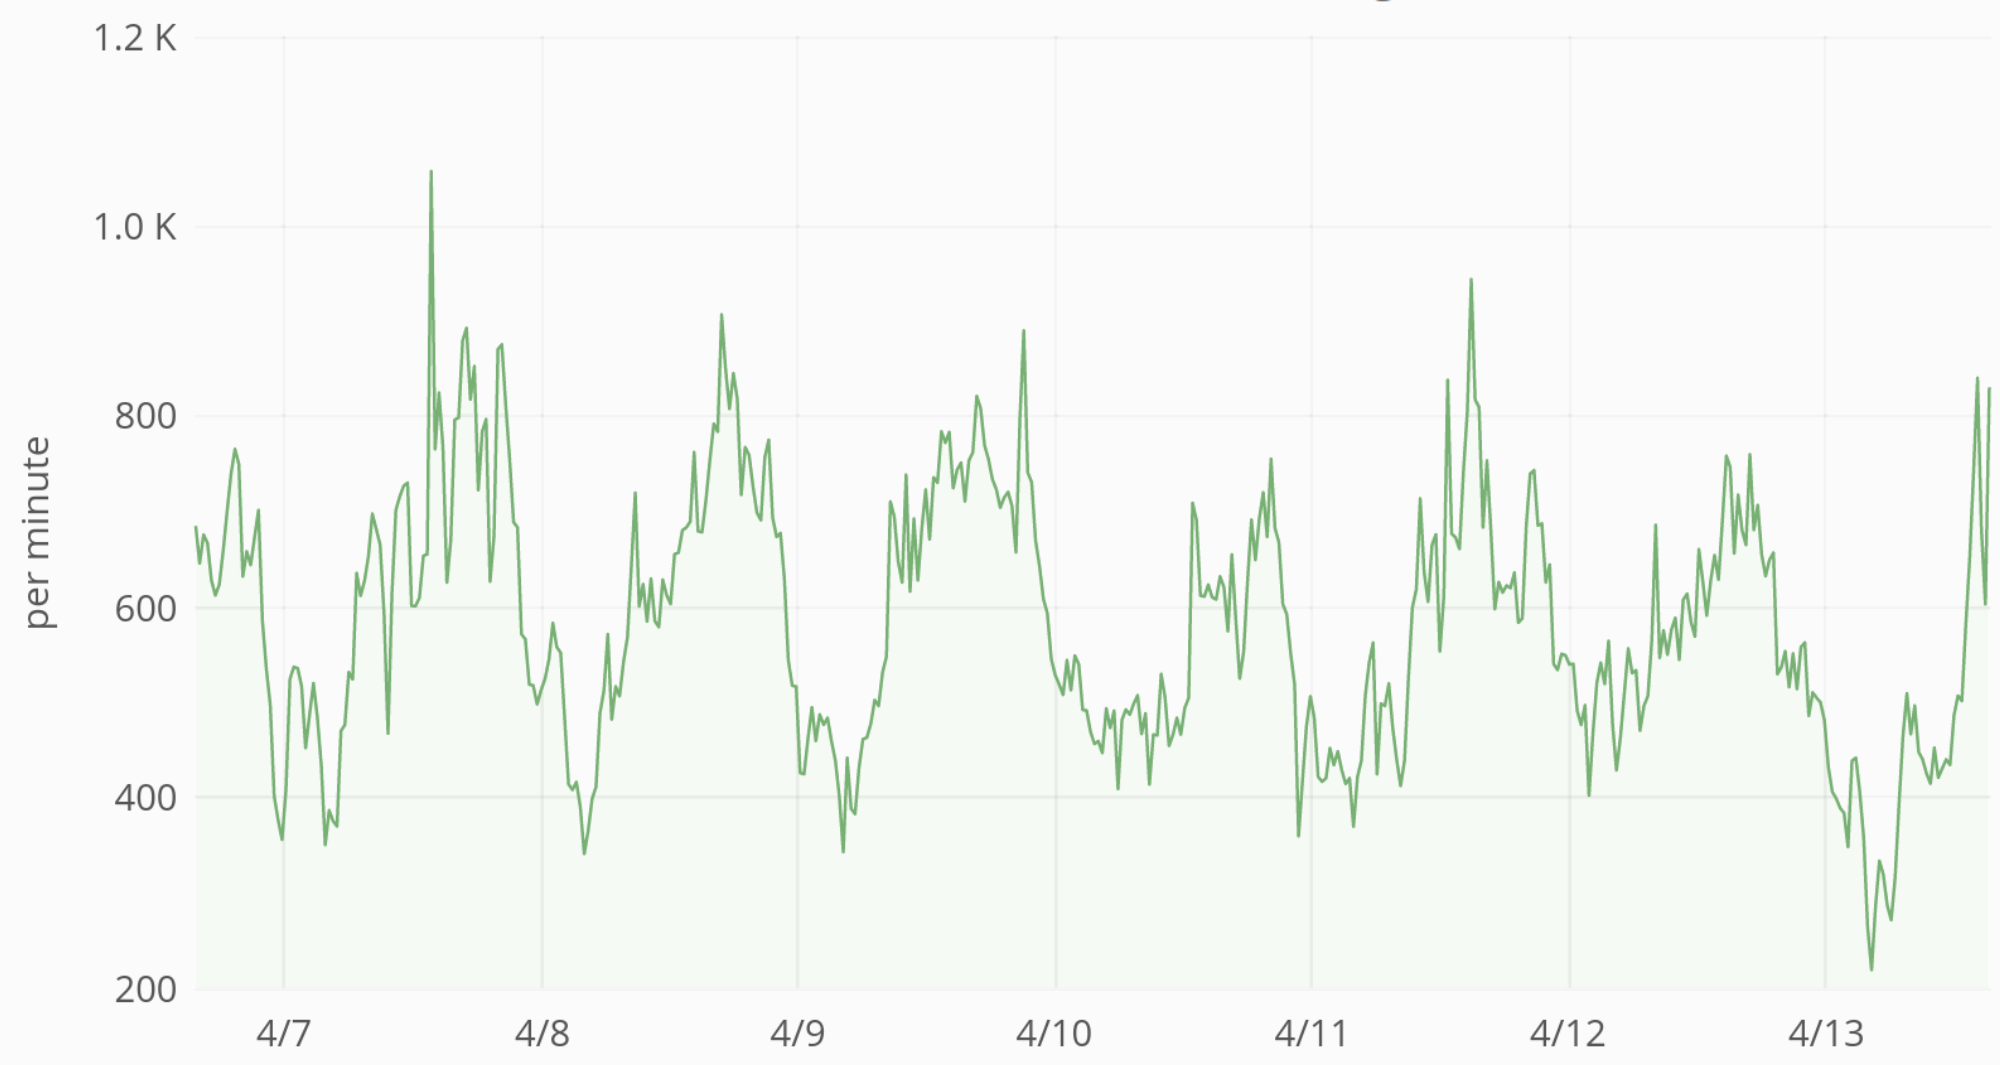
\includegraphics[width=.95\textwidth]{figures/ORES_precache_request_rate_201804}
  \caption{Precaching requests per minute}
  \label{fig:ores_precache_rate}
\end{subfigure}
\caption{Request rates to the ORES service for the week ending on April 13th, 2018}
\label{fig:ores_activity}
\end{figure}


The ORES service has been online since July 2015\cite{halfaker2015artificial}.  Since then, usage has steadily risen as we've developed and deployed new models and additional integrations are made by tool developers and researchers.  Currently, ORES supports 78 different models and 37 different language-specific wikis.

Generally, we see 50 to 125 requests per minute from external tools that are using ORES' predictions (excluding the MediaWiki extension that is more difficult to track).  Sometimes these external requests will burst up to 400-500 requests per second.  Figure~\ref{fig:ores_request_rate} shows the periodic and ``bursty'' nature of scoring requests received by the ORES service.  For example, every day at about 11:40 UTC, the request rate jumps---most likely a batch scoring job such as a bot.

Figure~\ref{fig:ores_precache_rate} shows the rate of precaching requests coming from our own systems.  This graph roughly reflects the rate of edits that are happening to all of the wikis that we support since we'll start a scoring job for nearly every edit as it happens.  Note that the number of precaching requests is about an order of magnitude higher than our known external score request rate.  This is expected, since Wikipedia editors and the tools they use will not request a score for every single revision.  This is a computational price we pay to attain a high cache hit rate and to ensure that our users get the quickest possible response for the scores that they \emph{do} need.

Taken together these strategies allow us to optimize the real-time quality control workflows and batch processing jobs of Wikipedians and their tools.  Without serious effort to make sure that ORES is practically fast and highly available to real-time use cases, ORES would become irrelevant to the target audience and thus irrelevant as a boundary-lowering intervention.  By engineering a system that conforms to the work-process needs of Wikipedians and their tools, we've built a systems intervention that has the potential gain wide adoption in Wikipedia's technical ecology.

\subsection{Explicit pipelines}
\label{sec:appendix.explicit_pipelines}
We have designed the process of training and deploying ORES prediction models to be repeatable and reviewable.  Consider the code shown in figure~\ref{fig:english_damaging_makefile} that represents a common pattern from our model-building Makefiles.

Essentially, this code helps someone determine where the labeled data comes from (manually labeled via the Wiki Labels system).  It makes it clear how features are extracted (using the \texttt{revscoring extract} utility and the \texttt{feature\_lists.enwiki.damaging} feature set).  Finally, this dataset of extracted features is used to cross-validate and train a model predicting the ``damaging'' label and a serialized version of that model is written to a file.  A user could clone this repository, install the set of requirements, and run \texttt{make enwiki\_models} and expect that all of the data-pipeline would be reproduced, and an equivalent model obtained.

By explicitly using public resources and releasing our utilities and Makefile source code under an open license (MIT), we have essentially implemented a turn-key process for replicating our model building and evaluation pipeline.  A developer can review this pipeline for issues knowing that they are not missing a step of the process because all steps are captured in the Makefile.  They can also build on the process (e.g. add new features) incrementally and restart the pipeline.  In our own experience, this explicit pipeline is extremely useful for identifying the origin of our own model building bugs and for making incremental improvements to ORES' models.

At the very base of our Makefile, a user can run \texttt{make models} to rebuild all of the models of a certain type.  We regularly perform this process ourselves to ensure that the Makefile is an accurate representation of the data flow pipeline.  Performing complete rebuild is essential when a breaking change is made to one of our libraries.  The resulting serialized models are saved to the source code repository so that a developer can review the history of any specific model and even experiment with generating scores using old model versions.

\begin{figure}[h]
        \makebox{\hrulefill}{
        \small
        \begin{verbatim}
datasets/enwiki.human_labeled_revisions.20k_2015.json:
    ./utility fetch_labels \
        https://labels.wmflabs.org/campaigns/enwiki/4/ > $@

datasets/enwiki.labeled_revisions.w_cache.20k_2015.json: \
        datasets/enwiki.labeled_revisions.20k_2015.json
    cat $< | \
        revscoring extract \
            editquality.feature_lists.enwiki.damaging \
            --host https://en.wikipedia.org \
            --extractor $(max_extractors) \
            --verbose > $@

models/enwiki.damaging.gradient_boosting.model: \
        datasets/enwiki.labeled_revisions.w_cache.20k_2015.json
    cat $^ | \
    revscoring cv_train \
        revscoring.scoring.models.GradientBoosting \
        editquality.feature_lists.enwiki.damaging \
        damaging \
        --version=$(damaging_major_minor).0 \
        -p 'learning_rate=0.01' \
        -p 'max_depth=7' \
        -p 'max_features="log2"' \
        -p 'n_estimators=700' \
        --label-weight $(damaging_weight) \
        --pop-rate "true=0.034163555464634586" \
        --pop-rate "false=0.9658364445353654" \
        --center --scale > $@
        \end{verbatim}
        \hrule
        \normalsize}
        \caption{Makefile rules for the English damage detection model from \url{https://github.com/wiki-ai/editquality}}
        \label{fig:english_damaging_makefile}
\end{figure}